\chapter{Trigger Types}
\label{chap:triggers}

There are five primary trigger types currently implemented in the \gls{deap3} firmware: periodic, exponential, external, minimum bias, and the ADC trigger. The trigger types, operation, and user settings are discussed below. More on the \gls{odb} can be found in Section \ref{sec:odb} with the settings and variable descriptions in the \href{https://www.snolab.ca/deap/private/TWiki/bin/view/Main/Dtmodb}{twiki}. This chapter borrows from the \href{https://www.snolab.ca/deap/private/TWiki/bin/view/Main/Triggerproject}{twiki, the link to which can be found here}.

\NOTE{Simulation information can be found on the \hypNote{twiki}{https://www.snolab.ca/deap/private/TWiki/bin/view/Main/FirmwareSimulation}}
\section{Periodic}
\label{sec:periodicTrigger}

\begin{description}
\item[SVN Location: ]https://edev.triumf.ca/svn/edevel00261/trunk/tsb/ip/rtl/source/ts\_periodic.v
\item[Module Name: ]TriggerSourcePeriodic
\item[Frequency Range: ]1 Hz $\rightarrow$ 100 kHz
\item[Submodules: ]None
\item[Summary: ]Used for testing the \gls{daq} system with a periodic signal (fixed interval between triggers). Uses a 100 kHz \gls{pll} and a counter to divide the rate. This trigger does not have a separate module, but is included in the \gls{vme} wrapper in edevel00270\footnotemark[\value{footnote}]. The periodic trigger has two identical channels used for the \gls{ppg} pulse injection, \gls{aarf} firing, status updates, etc.
\end{description}

\begin{landscape}
	\vspace*{\fill}
	\begin{figure}[ht]
	\centering
	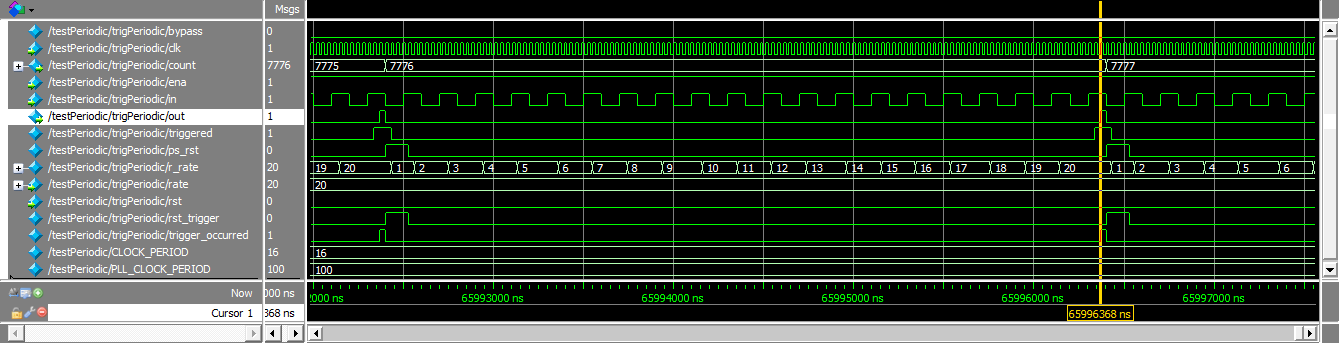
\includegraphics[width = \paperwidth]{periodicSim.png}
	\caption{Timing diagram for the periodic trigger.}
	\label{Fig:periodicTime}
	\end{figure}
	\vspace*{\fill}
\end{landscape}

\subsection{ODB Settings}
\label{sec:periodicODB}

\begin{figure}[ht]
\centering
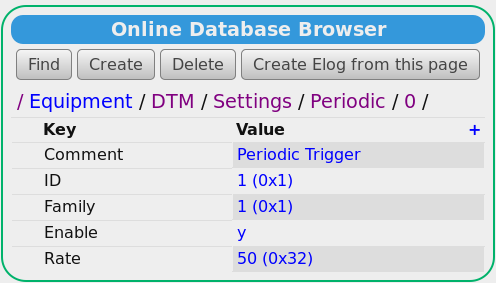
\includegraphics[width = 0.5\paperwidth]{periodicODB}
\caption{Online data base settings for the periodic trigger.}
label{Fig:periodicODB}
\end{figure}

\begin{description}
\item \textbf{Trigger ID: } Two identical channels
	\begin{description}
	\item \textbf{Channel 0: }0x1
	\item \textbf{Channel 1: }0xFFFFFFFF
	\end{description}

\item \textbf{Family: } 0x1 (Periodic)

\item \textbf{Enable: }Turns the trigger module on/off

\item \textbf{Rate: }Set rate of the trigger in Hz (1 $\rightarrow$ 10$^5$ Hz)
\end{description}

\section{Exponential}


\begin{description}
\item[SVN Location: ]https://edev.triumf.ca/svn/edevel00261/trunk/tsb/ip/rtl/source/ts\_exponential.v
\item[Module Name: ]TriggerSourceExponential
\item[Frequency Range: ]1 Hz $\rightarrow$ 62.5 MHz
\item[Submodules: ]None
\item[Summary: ] Used for testing the \gls{daq} system with exponentially distributed random intervals between triggers. Can emulate LAr background decay trigger rate, PMT dark noise trigger rate, expected event trigger rate $\rightarrow$ Emulates real \gls{daq} conditions. Uses a C++ program running on a NIOS core that generates the exponentially distributed random numbers for all 5 trigger sources, a FIFO to store those numbers and a counter that generates the trigger when the next random number is reached. The rate is more correctly the mean of the distribution from which delay times are taken, so the rate here is actually the time averaged rate.
\end{description}

\subsection{ODB Settings}
\label{sec:expODB}
\begin{figure}[ht]
\centering
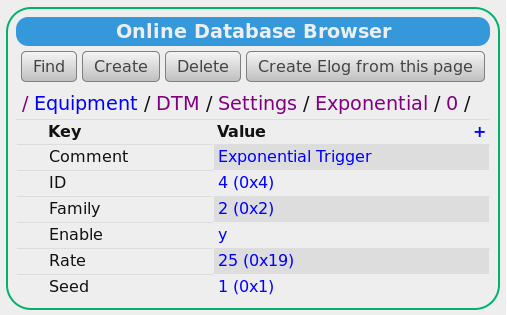
\includegraphics[width = 0.5\paperwidth]{expODB}
\caption{Online data base settings for the exponential trigger.}
\label{Fig:expODB}
\end{figure}
 

\begin{description}
\item \textbf{Trigger ID: } Five different identical channels
	\begin{description}
	\item \textbf{Channel 0: }0x4
	\item \textbf{Channel 1: }0x8
	\item \textbf{Channel 2: }0x10
	\item \textbf{Channel 3: }0x20 
	\item \textbf{Channel 4: }0x40 
	\end{description}

\item \textbf{Family: } 0x2 (Exponential)

\item \textbf{Enable: }Turns the trigger module on/off

\item \textbf{Rate: }Average rate of the trigger in Hz

\item \textbf{Seed: }Seed value for the random number generator
\end{description}
 
\section{External}
\begin{description}
\item[SVN Location:] https://edev.triumf.ca/svn/edevel00261/trunk/tsb/ip/rtl/source/ts\_external.v
\item[Module Name: ]TriggerSourceExternal
\item[Frequency Range: ] 0 Hz $\rightarrow$ 62.5 MHz (Pulses must be at least 16 ns wide)
\item[Submodules: ]None
\item[Summary: ]External triggers are sourced from the veto PMTs and the calibration devices via the \gls{nim} I/O \gls{fmc} (Section \ref{sec:nimBoard}). These external triggers are primarily intended for the removal of muon events which can be tagged by the veto system as they create Cerenkov radiation in the water tank. There are three identical channels, one for the veto system and two of which are currently unassigned\footnote{July 2016}.
\end{description}
\begin{landscape}
	\vspace*{\fill}
	\begin{figure}[ht]
	\centering
	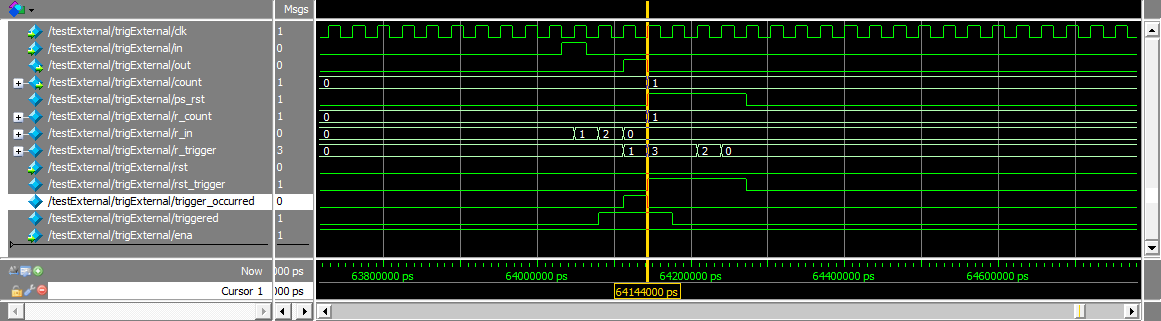
\includegraphics[width = \paperwidth]{externalSim.png}
	\caption{Timing diagram for the external trigger.}
	\label{Fig:}
	\end{figure}
	\vspace*{\fill}
\end{landscape}

\subsection{ODB Settings}
\label{sec:externalODB}

\begin{figure}[ht]
	\centering
	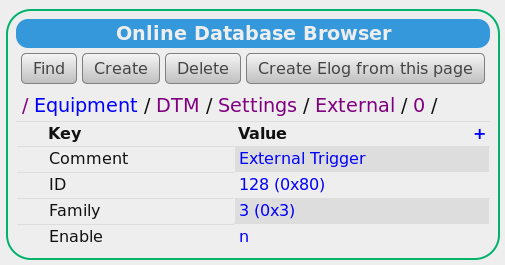
\includegraphics[width = 0.5\paperwidth]{externalODB}
	\caption{Online data base settings for the external trigger.}
	\label{Fig:externalODB}
\end{figure}


\begin{table}
	\centering
	\caption{Trigger ID and connections for the external trigger}
	\begin{tabular}{l l l l}
	Channel&	Trigger ID&		NIM Channel&	Application\\ \hline \hline	
			0&		0x80&				0&				Veto\\  
			1&		0x100&				1&				Calib\\ 
			2&		0x200&				2&				External Trigger 2\\ \hline \hline		
	\end{tabular}
\end{table}

\begin{description}
\item \textbf{Family: } 0x3 (External)

\item \textbf{Enable: }Turns the trigger module on/off
\end{description}

\section{Minimum Bias}
\label{sec:minBias}
\begin{description}
\item[SVN Location:] https://edev.triumf.ca/svn/edevel00261/trunk/tsb/ip/rtl/source/ts\_adc\_min\_bias.v
\item[Module Name: ]TriggerSourceADCMinimumBias
\item[Frequency Range: ]Settings Dependant, minimum time between triggering four clock delay (Reset and flip-flop setting) + dead time + \gls{tot} time (see Fig. \ref{Fig:minBiasSingleSim} and \ref{Fig:minBiasCoincSim})
\item[Submodules: ]min\_bias\_sum (channel counting megafunction)
\item[Summary: ]The minimum bias trigger compares the \gls{asum} data to a threshold set in the online data base \gls{odb}. If the signal stays above this threshold for a certain defined time known as the time over threshold (\gls{tot}), then the channel is said to have latched (diagram in Fig. \ref{Fig:minBiasTrigger}). The \gls{tot} requirement is intended to reduces the chance of triggering on noise.

There are two modes for the min. bias trigger: single channel or coincidence mode. In single channel mode, once one channel latches the trigger condition is met and a trigger signal is sent. In coincidence mode multiple channels need to latch within a definable amount of time known as the coincidence time window. In coincidence mode once the last channel has latched a trigger signal is sent. 

Once a trigger condition has been met and a trigger signal output, the trigger goes into a dead state until the defined deadtime has been passed. The deadtime is intended to reduce the chance of retriggering on the same event.
 
 \NOTE{The minimum bias can be used with the 22 \gls{asum} channels and the \gls{ass}, which channels are enabled are set in the \gls{odb}.}
 %In order to readout the \gls{dtm} ADC waveform data corresponding to the trigger, an ADC FREEZE FIFO LATENCY of about 2500 cycles (62.5 MHz) is required with the current FIFO settings. 
\end{description}

\begin{figure}[ht]
\centering
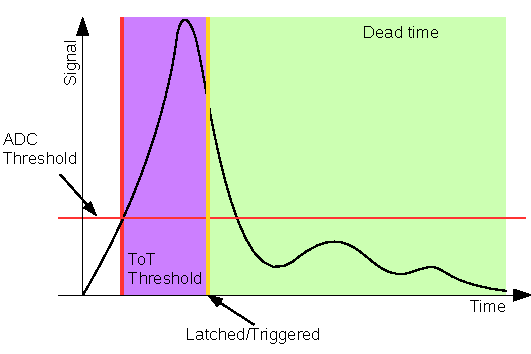
\includegraphics[width = 0.7\paperwidth]{minBiasTrigger.pdf}
\caption{Cartoon depicting the operation of the minimum bias trigger. The trigger fires once the signal has remained above the adc threshold (horizontal line) for the time over threshold (vertical red line) at which point the trigger will fire immediately (vertical yellow line). The trigger may not re-fire until the deadtime has been exceeded.}
\label{Fig:minBiasTrigger}
\end{figure}


\begin{landscape}
	\vspace*{\fill}
	\begin{figure}[ht]
	\centering
	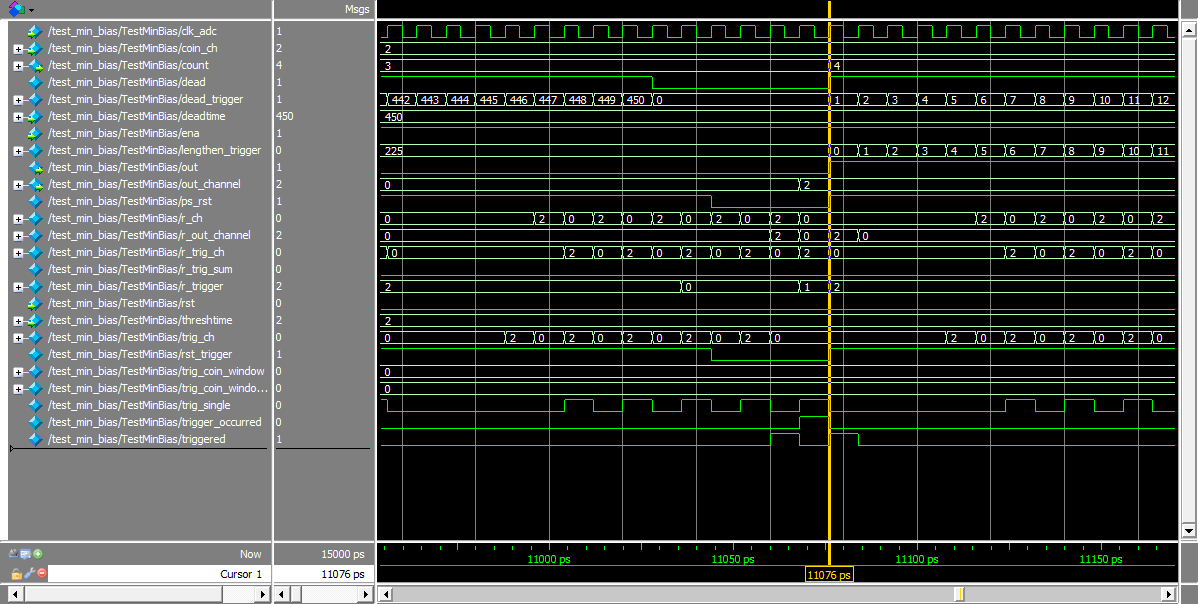
\includegraphics[width = \paperwidth]{minBiasSingleChannel.png}
	\caption{Timing diagram for the minimum bias trigger in single channel mode.}
	\label{Fig:minBiasSingleSim}
	\end{figure}
	\vspace*{\fill}
\end{landscape}

\begin{landscape}
\vspace*{\fill}
	\begin{figure}[ht]
	\centering
	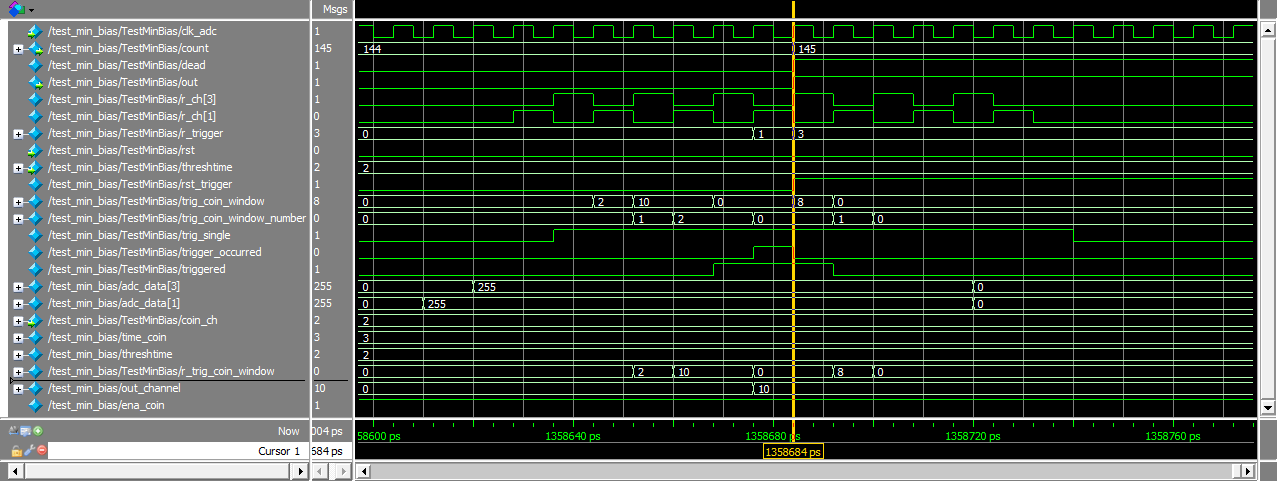
\includegraphics[width = \paperwidth]{minBiasCoincidence.png}
	\caption{Timing diagram for the minimum bias trigger in coincidence mode.}
	\label{Fig:minBiasCoincSim}
	\end{figure}
\vspace*{\fill}
\end{landscape}

\subsection{ODB Settings}
\label{sec:minBiasODB}
\begin{figure}[ht]
\centering
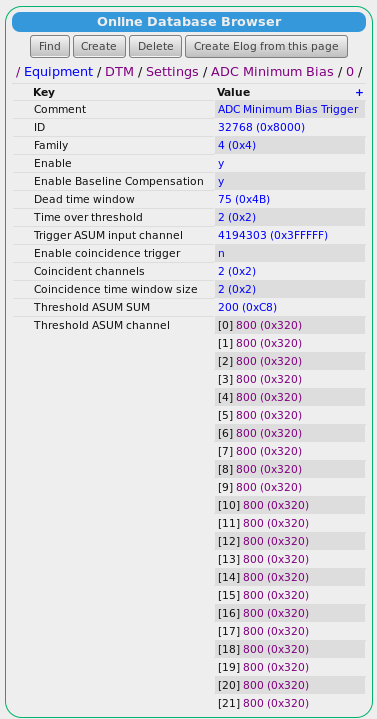
\includegraphics[height = 0.75\paperheight]{minBiasODB}
\caption{Online data base settings for the min. bias trigger.}
\label{Fig:minBiasODB}
\end{figure}

\begin{description}
\item \textbf{Trigger ID: } 0x8000

\item \textbf{Family: } 0x4 (Physics)

\item \textbf{Enable: }Turns the trigger module on/off

\item \textbf{Enable Baseline Compensation: }Will apply the baseline subtraction from the read ADC value. If enabled the thresholds will be used on the baseline subtracted reading.

\item \textbf{Dead Time Window: } 16-bit value which sets the number of clocks after a trigger event wherein no more triggers will be produced to avoid retrieving on the same event. (\NOTE{This should be significantly larger than the long time window}

\item \textbf{Time over Threshold: }16-bit value which sets the minimum number of clocks after a threshold has been crossed that the signal must remain high for a trigger to be produced. \NOTE{As this is used to only remove noise, the \gls{tot} is usually set at a only a few clocks}
 
\item \textbf{Trigger \gls{asum} input channel: } Bit mask for enabled channel inputs; a disabled channel has its corresponding bit set false. Bits 1-22 are the \gls{asum} channels and bit 23 is the \gls{ass}. Any combination can be enabled. 

\item \textbf{Coincident Channels: }Number of channels required to have fulfilled the triggering requirements within the coincident time window size if the coincidence trigger is enabled. For instance if this value is set to four, than within the coincidence time window size a minimum of 4 channels must have crossed their thresholds for a time greater than the \gls{tot} for a trigger to be produced.
	
\item \textbf{Coincident time window size: } 16-bit value which sets the number of clocks in the time window for the number of channels defined by the coincident channels setting to have each meant the single channel trigger requirements (only applies for coincidence trigger mode). 

\item \textbf{Threshold \gls{ass}: }17-bit value setting the minimum bias threshold for the \gls{ass}.

\item \textbf{Threshold \gls{asum} channel: }12-bit value setting the minimum bias threshold for each of the \gls{asum} channels.
\end{description}


\clearpage
\section{ADC Trigger}
\label{sec:adcTrig}
\begin{description}
\item[SVN Location: ]https://edev.triumf.ca/svn/edevel00261/trunk/tsb/ip/rtl/source/ts\_adc.v
\item[Module Name: ]TriggerSourceADC
\item[Frequency Range: ]Settings Dependant, minimum time between triggering five clock delay (reset and flip-flop setting) + dead time + scan time\footnote{Scan time in the \gls{odb}, look ahead time in the literature, the firmware variable in the timing diagram is 'waittime'} (See Fig. \ref{Fig:adcSim})
\item[Submodules: ]trigger\_self\_sum\_adc (see Section \ref{sec:selfSum}), TriggerSelfDecision (see Section \ref{sec:trigSelfDecision})
\item[Summary: ]The ADC trigger receives the baseline subtracted \gls{ass} and analyzes the short energy and \gls{fprompt} to make a triggering decision. The module trigger\_self\_sum (Section \ref{sec:selfSum}) performs a rolling integral over a short ($\sim$8 clocks)\footnote{This module uses the ADC clock of 45.161290 MHz} and a long time window ($\sim$150 clocks) as shown in Fig. \ref{Fig:adcTrigger}. The short integration window integral is delayed to be valid at the same time as the long window (see Section \ref{sec:selfSum}) so the decision is always made after the integration of both windows is finished.

The integrals are passed to the module TriggerSelfDecision (Section \ref{sec:trigSelfDecision}) which dynamically sorts 'events' into one of six groups as shown in Fig. \ref{Fig:triggerRegions}. If the charge in the short window exceeds the low energy limit, then a variable 'trig\_out' is set as shown in Fig. \ref{Fig:bitFieldADCTrig} (colours and bit positions are consistent with Fig. \ref{Fig:triggerRegions}). If the value of trig\_out increase (i.e. higher \gls{fprompt} or short charge) or stays the same with the energy increasing, the values from that time are saved and the comparison continues. If The value of trig\_out decreases or stays the same with the short energy decreasing or staying the same, then an \gls{odb} defined timer referred to as the look ahead time \footnote{this is called the scan time in the \gls{odb}, waittime in the firmware, or look ahead time in some documentation} ($\sim$15 clocks) begins counting. If a value of trig\_out of the same or greater value is found within this look ahead time, then that the values (short/long window charge, trigger type, and trigger start time, etc.) are set to the new events and the timer is restarted\footnote{If a second maxima is found in the look ahead time of equal or greater charge than the first, the scan time will start again from that point and the reported trigger will be of the last maxima.}. Only once the timer reaches the look ahead time without finding a higher value of trig\_out is a trigger produced.

\begin{figure}[ht]
\centering
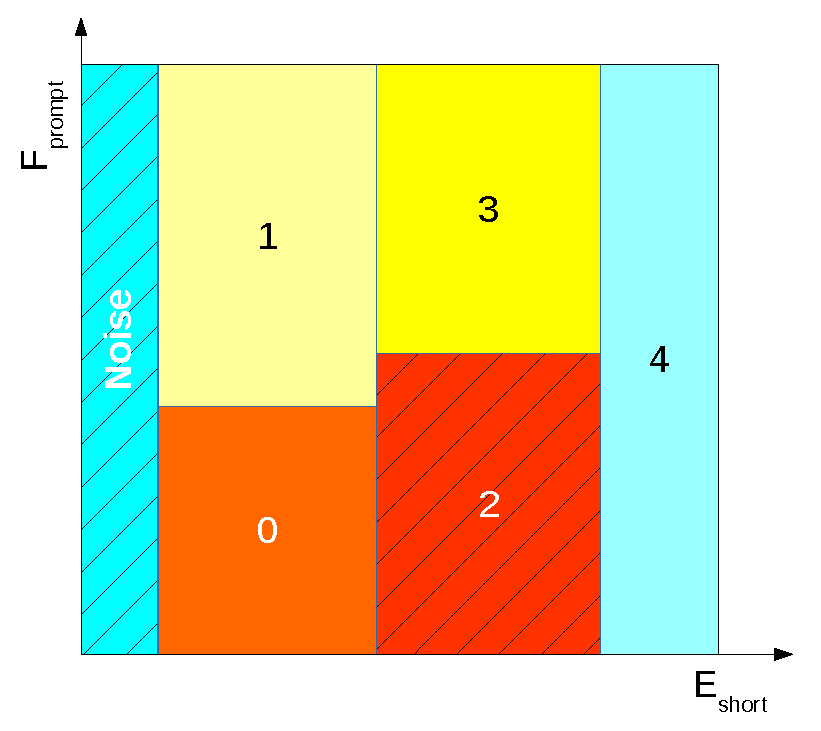
\includegraphics[width = 0.6\paperwidth]{triggerRegions}
\caption{Trigger regions as used in the pulse shape discrimination background rejection method. Noise in the \gls{pmt}s fall under very low energy and $\beta$ events are grouped into high energy, low \gls{fprompt}. The \gls{wimp} region of interest is at high \gls{fprompt} and could fall into either region of energy.}
\label{Fig:triggerRegions}
\end{figure}

\definecolor{orange}{rgb}{1.8,1,.1}
\begin{figure}
	\begin{bytefield}[endianness=big, bitheight=3.0\baselineskip]{30}
	\colorbitbox{webblue}{6}{Very High\\Energy\\Bit 4}
	\colorbitbox{yellow}{6}{High Energy\\High Fprompt\\Bit 3}
	\colorbitbox{red}{6}{High Energy\\Low Fprompt\\Bit 2}
	\colorbitbox{orange}{6}{Low Energy\\High Fprompt\\Bit 1}  
	\colorbitbox{webred}{6}{Low Energy\\Low Fprompt\\Bit 0}
	\end{bytefield}
	\caption{trig\_out variable, the higher the charge and \gls{fprompt}, the higher the value. Values and colours correspond to the regions shown in Fig. \ref{Fig:triggerRegions}.}
	\label{Fig:bitFieldADCTrig}
\end{figure}

\end{description} 
\begin{figure}[ht]
\centering
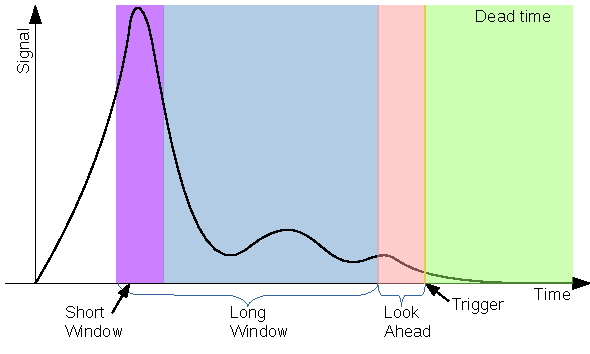
\includegraphics[width = 0.7\paperwidth]{adcTrigger}
\caption{Short and long time integration windows for the determination of the fraction of prompt charge in an event (\gls{fprompt}).}
\label{Fig:adcTrigger}
\end{figure}

The \gls{fprompt} is not explicitly calculated however it is used for event selection; for a defined \gls{fprompt} (for 1$<$F$_{\text{thres}}< 256$) an event is recorded if:

\begin{equation}
\text{E}_{\text{long}} > \text{E}_{\text{thres}} \ \& \ \text{E}_{\text{long}} \times \text{F}_{\text{thres}} >\left[ \text{E}_{\text{short}} \times 256\right].
\label{Eq:fpromptDecision} 
\end{equation}
Thus if a \gls{fprompt} of 0.5 is desired, the \gls{odb} value is set to F$_{\text{thres}} = (256 \times 0.5) = 128$. Events are sorted using the short energy and \gls{fprompt} into one of five regions as depicted in Fig. \ref{Fig:triggerRegions} (region 0 is defined as below threshold therefore nothing is recorded).

After a trigger signal has been generated the trigger will enter a dead state where no triggering is allowed. This dead time is implemented so as to avoid retriggering on the same event\footnote{Note that the scan time adds to the dead time for the minimum time between triggers}. A diagram of the ADC trigger is given in Fig. \ref{Fig:adcTrigger}. 

\NOTE{The look ahead time does occur after the long window finishes integrating, but as the short and long window times are valid at the same time due to a delay fifo, the look ahead time applies 'back in time' if you will with regards to Fig. \ref{Fig:adcTrigger}}. A full timing diagram of the ADC trigger while constantly triggering is shown in Fig. \ref{Fig:adcSim}. 

\begin{landscape}
	\vspace*{\fill}
	\begin{figure}[ht]
	\centering
	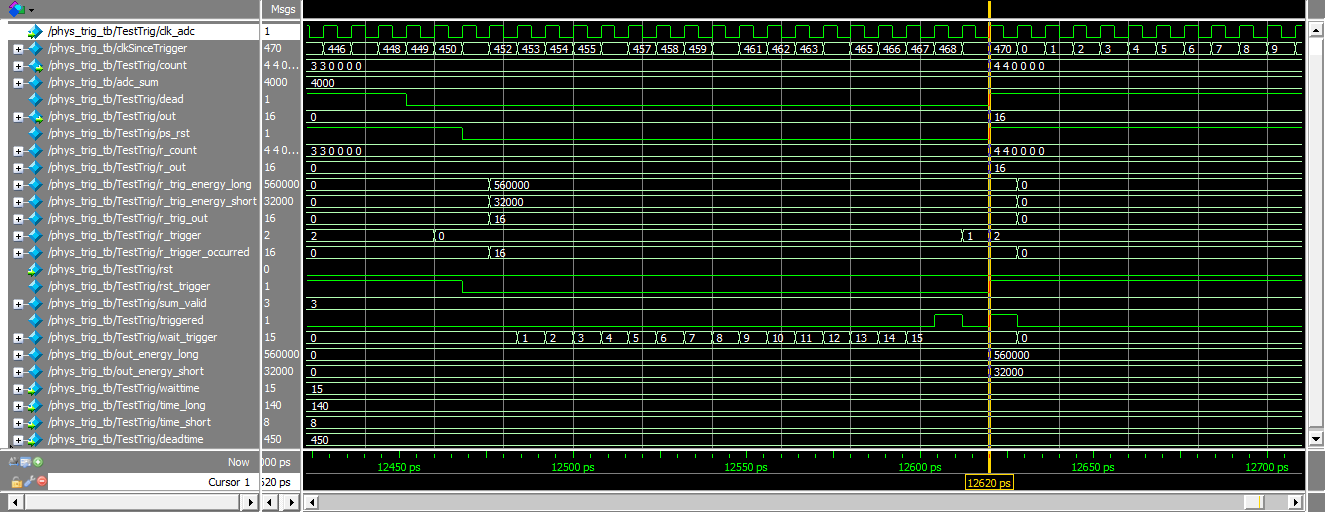
\includegraphics[width = \paperwidth]{adcTrigSim.png}
	\caption{Timing diagram for the ADC trigger at constant triggering.}
	\label{Fig:adcSim}
	\end{figure}
	\vspace*{\fill}
\end{landscape}


\subsection{ODB Settings}
\label{sec:adcTrigODB}
\begin{figure}[ht]
\centering
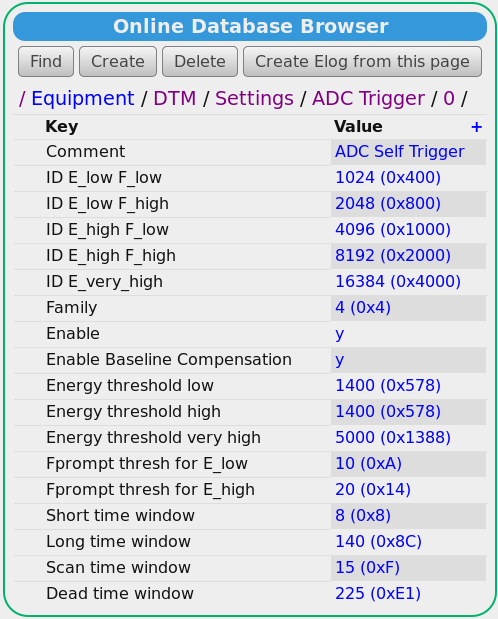
\includegraphics[width = 0.5\paperwidth]{adcTrigODB}
\caption{Online data base settings for the ADC trigger.}
\label{Fig:adcTrigODB}
\end{figure}

\begin{description}

\item \textbf{Trigger ID: } The ADC trigger has only a single channel but has 5 trigger IDs corresponding to the five zones depicted in Fig. \ref{Fig:triggerRegions}. These trigger types are taken from trig\_adc depicted in Fig. \ref{Fig:bitFieldADCTrig}.
	\begin{description}
	\item \textbf{Zone 0}: 0x400
	\item \textbf{Zone 1}: 0x800
	\item \textbf{Zone 2}: 0x1000
	\item \textbf{Zone 3}: 0x2000
	\item \textbf{Zone 4}: 0x4000
	\end{description}

\item \textbf{Family: }0x4 (Physics)

\item \textbf{Enable: }Turns the trigger module on/off

\item \textbf{Enable Baseline Compensation: }Will apply the baseline subtraction from the read ADC value. If disabled the thresholds will be used on the baseline subtracted reading. \NOTE{The \gls{fprompt} is nonsensical with this disabled.}

\item \textbf{Energy Thresholds: }17-bit value (sum of 22 12-bit \gls{asum}s). If the baseline subtraction is enabled then the thresholds are taken from the subtracted reading.
	\begin{description}
	\item \textbf{Low: }Cutoff between noise and zones 0/1
	\item \textbf{High: }Cutoff between zones 0/1 and zones 2/3
	\item \textbf{Very High: }Cutoff between noise zones 2/3 and zone 4 
	\end{description}

\item \textbf{\gls{fprompt} Thresholds: }Cutoff between low and high \gls{fprompt}. \gls{fprompt} is given as an eight bit value, trigger decisions follow Eq. \eqref{Eq:fpromptDecision}.
	\begin{description}
	\item \textbf{Low Energy: }\gls{fprompt} separation between zones 0 and 1
	\item \textbf{High Energy: }\gls{fprompt} separation between zones 2 and 3
	\end{description} 
	
\item \textbf{Short Time Window: } 1-50 value (1.1 $\mu$s) which sets the number of clocks the charge in the short integration window (see Fig. \ref{Fig:adcTrigger})

\item \textbf{Long Time Window: }1-500 value (11 $\mu$s) which sets the number of clocks the charge in the long integration window (see Fig. \ref{Fig:adcTrigger})

\item \textbf{Scan Time Window: }16-bit value which sets the number of clocks to look to see if the currently found maxima is local or general (within the scan time). The scan time is intended to ensure that the integrated value of the short window is maximized.

\item \textbf{Dead Time Window: }16-bit value which sets the number of clocks after a trigger event wherein no more triggers will be produced to avoid retriggering on the same event. \NOTE{This should be significantly larger than the long time window.}

\end{description}

\section{ODB}
\label{sec:odb}
The online data base (\gls{odb}) contains all of the controls and settings for the triggers on a webpage. More information on the \gls{odb} can be found \hypNote{on the \gls{midas} site}{https://midas.triumf.ca/MidasWiki/index.php/Online_Database}.


The \gls{dtm} \gls{odb} settings can be found in their entirety on the \hypNote{twiki}{https://www.snolab.ca/deap/private/TWiki/bin/view/Main/Dtmodb}
